%%
%%
%% aux_doxygen.tex for  in cours/outils_gnu
%%
%% Made by Philippe THIERRY
%% Login   <Philippe THIERRYreseau-libre.net>
%%
%% Started on  sam. 18 sept. 2010 11:52:02 CEST Philippe THIERRY
%% Last update sam. 18 sept. 2010 12:20:09 CEST Philippe THIERRY
%%

\chapter{Exemple d'utilisation de commentaires Doxygen dans le code}

\paragraph{}
Le script \ref{lst:doxygen_example} est un extrait d'un exemple r�el d'utilisation de doxygen pour
g�n�rer un document \LaTeX, puis PDF apr�s compilation. Les images \ref{pic:doxy_output_1} et
\ref{pic:dpxy_output_2} montrent un extrait du fichier PDF g�n�r� avec le document source \ref{lst:doxygen_example}.

\begin{lstlisting}[caption={Exemple d'utilisation de Doxygen dans un source C},label=lst:doxygen_example]
/*
** File cm_libdebug.h for project libcommon
**
** Made by Jean-Marc LACROIX
** Login   <jeanmarc.lacroix@free.fr>
**
** Copyright (C) 2009 - Jean-Marc LACROIX
**
** This program is  free   software; you can redistribute  it   and/or
** modify it under the terms of the  GNU Lesser General Public License
** as published  by the Free  Software Foundation; either version 2 of
** the License, or (at your option) any later version.
**
** This program is distributed in the hope that it will be useful, but
** WITHOUT  ANY  WARRANTY; without    even the  implied  warranty   of
** MERCHANTABILITY or  FITNESS FOR A PARTICULAR  PURPOSE.  See the GNU
** General Public License for more details.
**
** You should have received a  copy of the  GNU General Public License
** along  with   this program;  if  not, write  to the   Free Software
** Foundation, Inc.,  59   Temple  Place   - Suite  330,  Boston,   MA
** 02111-1307, USA.
*/

/*!
** \file cm_libdebug.h
**
** \abstract
**
** This file contains  API for libdebug library. It  should be used by
** whatever   software  using   this  lib.    This library  implements
** different capacities of debugging, warning, erroring and offers the
** possibility to send output trace/debug message on different devices
** such syslog, file, socket ...
**
** The purpose of the API is to  offer a simple interface for printing
** and debugging   informations in  user  applications  with  only one
** macro:  CM_DBG_TRACE.  This macro  is a  frontend of 'fprintf' with
** following improvements and features :
**
**    - 1 - Output format : The ouput format is variadic type, so that
**    all printf format specification is  supported .  Furthermore, in
**    order  to support also   debugging,  the macro  incorporate  the
**    standard C99 __LINE__, __FILE__ and  __func__ macro , so that it
**    is  possible to improve  debugging  and trace  in  a application
**    without  modifying the code.  All  this  aspects are embedded in
**    the CM_DBG_TRACE macro.
**
**    -  2 - Output  device : in order to  send output trace and debug
**    informations, the   device on which  all traffic  is sent can be
**    choosed   by  user    at startup   time  during   initialisation
**    phase. Different kind of device are allowed, such :
**
**         - standard file
**         - standard BSD syslog API
**         - UDP IPV4 unicast socket
**         - TCP IPV4 unicast socket
**         - device STDOUT
**         - device STDERR
**
**    - 3 - Dynamic management: the output format can be change at run
**    time without  changing or recompiling application.  For exemple,
**    at startup time,  the default value  can be only to edit message
**    on syslog, and later, a API is available to change the format by
**    adding __FILE__ and/or other characteristics. This management is
**    implemented with state machine so that there are no interruption
**    in debug data flow.
**
**    - 4  -  Real time aspect: All   ressources reservation  are done
**    during   initialisation phase, so   no   memory nor  thread  are
**    allocated during normal life of API.
**
**    - 5 - End to end  communication: When sending debug and/or trace
**    on a system, it is some time critical  to be sure that integrity
**    of the  session is correct  bettween message n  and message n+1.
**    In  order to do  that, a  prefix counter (  like other  __LINE__
**    prefix  ) is available  and  can be  used / unused  dynamically.
**    This counter is 32 bit wide and is / is not in all messages.  It
**    is user responsabilitie to verify coherence bettween message (n)
**    and message (n+1).  This behavior can  help when sending message
**    on UDP protocol for exemple for detection on broken message when
**    a message is  dropped by  the  network (for integrity point   of
**    view).  It implement a 'session' counter mechanism with a simple
**    algorythm:  (counter   ++),  so that   end  point  communication
**    application can verify correct transmission.
**
**    -  6 - Date  prefix: On complex network system,  it is some time
**    mandatory to have  date  information on event message   from the
**    origin    daemon  with   high    occuracy.   Of   course  Syslog
**    implementation  (sylogd/syslog_ng)  install  local date  on each
**    event/message, and, with this feature, it  is possible to manage
**    complex  network if syslogd daemon is  present.  But at the same
**    time,   syslog is used  with a  resolution about  second, and in
**    order to  have  a datation with  more  occuracy , it  is not the
**    solution. Furthermore, the datation is done from syslogd daemon,
**    not from initial daemon logger  end point.This API incorporate a
**    similar  mechanism in order to   install a date  pattern on each
**    line event message.  In order to  minimize real time impact when
**    getting date on local system, no  Posix time API is used because
**    overhead can  not be supported  on embbeded system, and also due
**    to the fact that there are cases on which rescheduling can occur
**    when getting date.  The proposal implementation is to use a very
**    light 'date' API based on new hardware feature available on most
**    todays platform.   This feature is know  as 'rdtsc' on X86/IA32,
**    but exist  also on ARM, PPC  and other MIPS architecture.  It is
**    often a hardware counter running at CPU  clock or near.  The bad
**    news is that this feature is not  normalize and as a consequence
**    hardware dependant.   Furthermore, it  depends of the  CPU clock
**    (please  care   must  be  taken   on   laptop  system).  Another
**    disavantage of this   mechanism  is that  getting date  is   not
**    synchronize   with any  other  system  such as   NTP,   and as a
**    consequence, the validity of  time is only local,  but it is the
**    MAJOR  requirement.  The good  news is as this implementation is
**    very light,  it is  possible to  have  extreme occuracy on event
**    datation message.  Please look  at libcommn 'cycle' component in
**    order to have more informations.  On  modern system, the 'rdtsc'
**    counter is  very often a 64 bits  counter, so the format used in
**    this feature  is  simpler 64  bits  long  (\%lld) ,  it is  user
**    responsabilitie to   manage  this  information and  make   other
**    correlation  or  treatment    on  the  data    flow produced  by
**    CM_DBG_TRACE.   As a conclusion,  this feature  is one option as
**    the others format  options  and must  be used  in case  of  high
**    occuracy.
**
**    - 7 - Thread safe. No thread  are used in this  API, and also no
**    lock, mutex or other synchronisation mechanisms are used.
**
**    - 8 -  Non blocking mode: some  time, when using monoprocess  or
**    monothread applications, it is mandatory to never block in order
**    to be  sure to  manage correctly input  traffic  on 'select' (or
**    equivalent) synchronisation   point.  In order  to  be compliant
**    with  this requirement, the  API  offer a double  mechanism when
**    using  output traffic  on  TCP  socket.  First  is the  standard
**    native Posix blocking mode in which all call to CM_DBG_TRACE are
**    synchronous, and of course, some time, this call block depending
**    of TCP windows and  length of SO_SNDBUF   buffer socket in  your
**    application.  Second is  the possibility to used CM_DBG_TRACE in
**    a non blocking mode on TCP protocol.   Of course, in order to do
**    that, a    local  buffer  must be    preallocated  (only  during
**    initialisation  phase)   and output  traffic  is  write  to this
**    buffer.  In  this case, it   is user  responsabilitie to  manage
**    later  this  traffic buffer   with a   Posix 'select'  or  other
**    equivalent mechanism.  Furthermore, is is also possible for user
**    to choose SO_SNDBUF Posix option  parameter.  To end about  this
**    feature, the last (but not least) is  the ability to support non
**    blocking mode when creating output traffic  with SYN TCP packet.
**    In  this case,  a timeout  can be  choosen  in order  to overlap
**    standard  Operating System parameter.    Please note  this  last
**    feature never use /proc or  /sys OS parameter,  it is only based
**    on  standard Posix non  blocking  socket API.  Please  note that
**    'non blocking mode' is under development.
**
** Before  calling any of libdebug services,  it is  mandatory to call
** only once cm_debug_init,  otherwise all services respond with error
** code ( conform to REQ_SOFT_ARCH_0060 )
**
** \dependencies
**
** The  'debug'    LIBCOMMON module use    module  'cycles' and module
** 'socket'.  This 2 modules   are used until  cm_libdebug_release  ()
** service is called. Furthermore, during initialisation phase, module
** 'version' is initialised and released  for cm_debug_init() and also
** for cm_debug_release() service.
**
** \author Jean-Marc LACROIX
**
** \version initial version
**
** \date September 2009
**
** \requirements
** This file is compliant with the following requirements :
** ( look at manual )
** REQ_CODE_QUALITY_0020
** REQ_CODE_QUALITY_0060
** REQ_CODE_QUALITY_0080
** REQ_CODE_QUALITY_0090
** REQ_CODE_QUALITY_0130
** REQ_SOFT_ARCH_0020
** REQ_SOFT_ARCH_0030
** REQ_SOFT_ARCH_0060
** REQ_SOFT_ARCH_0090
*/

#include <netdb.h>

#ifndef LIBDEBUG_H_
# define LIBDEBUG_H_

#include <stdlib.h>
#include <unistd.h>
#include <stdio.h>
#include <inttypes.h>
#include <ctype.h>
#include <sys/types.h>
#include <stdint.h>
#include <string.h>
#include <signal.h>
#include <time.h>
#include <syslog.h>

#include "cm_libtypes.h"
#include "cm_libsocket.h"

/*!
**
** \brief CM_DBG_MAX_PREFIX_SIZE  : maximum length for internal prefix
** representation (local static allocation)
*/
#define CM_DBG_MAX_PREFIX_SIZE	  30
/*!
**
** \brief CM_DBG_MAX_SIZE_BUFFER : maximum  length for internal buffer
** representation (local static allocation)
*/
#define CM_DBG_MAX_SIZE_BUFFER    512
/*!
**
** \brief CM_DBG_LAST_MESSAGE : define  the last  message in log  when
** closing device
*/
#define CM_DBG_LAST_MESSAGE       "libcommon_last_message"
/*!
**
** \brief CM_DBG_FIRST_MESSAGE : define the  first message in log when
** opening device
*/
#define CM_DBG_FIRST_MESSAGE      "libcommon_first_message"
/*!
**
** \brief  CM_DBG_DEFAULT_PREFIX : the default  prefix when user don't
** specify a prefix or when user prefix is invalid
*/
#define CM_DBG_DEFAULT_PREFIX     "cm_libdebug_prefix"
/*!
**
** \brief CM_DBG_BAD_SEVERITY_VALUE  : a  string in order  to indicate
** error
*/
#define CM_DBG_BAD_SEVERITY_VALUE "BAD-RFC" /**<         used       by
					  cm_debug_severity_get_string  */
/*!
**
** @brief This enum describe the different severities of debugging.
**
** It is   compliant to RFC3164    (table 2).  Of   course  there is a
** hierarchy in this  definition, so it is  the responsability of user
** to  use this  enumerate  with correct  severity according  expected
** behaviour.
*/
typedef enum
{
  CM_E_DBG_SEVERITY_PANIC,     /**< system is unusable */
  CM_E_DBG_SEVERITY_ALERT,     /**< action must be taken immediatly*/
  CM_E_DBG_SEVERITY_CRIT,      /**< critical conditions */
  CM_E_DBG_SEVERITY_ERROR,     /**< error conditions*/
  CM_E_DBG_SEVERITY_WARNING,   /**< warning conditions */
  CM_E_DBG_SEVERITY_NOTICE,    /**< normal but signifiant notice */
  CM_E_DBG_SEVERITY_INFO,      /**< simple informational */
  CM_E_DBG_SEVERITY_DEBUG,     /**< debug-severity message */
  CM_E_DBG_SEVERITY_MAX        /**< max  value. also used  for invalid
								  value and   for sizing  this object,
								  not available for user  */
} cm_e_dbg_severity;

[...]

/*!
**
** @brief The service cm_debug_device_change() is  used to change  the
** type of device : deprecated,  please close and reopen, this service
** must be suppressed as soon as possible.
**
** This service change current device to  new specified device.  It is
** assume  that  user has  previously  close  the current  device with
** cm_debug_release,   otherwise,   some  buffer  information  can  be
** droppped !!
**
** @param device_type define the new device to use.  if device_type >=
** CM_E_DBG_DEV_MAX,    then  local    initialisation   is   made   to
** CM_E_DBG_DEV_MAX value and returning is done to CM_E_TYPE_RET_ERROR
** in order to indicate a bad input value
**
** @return     CM_E_TYPE_RET_OK if  successful,    CM_E_TYPE_RET_ERROR
** otherwise
*/
cm_e_type_ret_value
cm_debug_device_change(cm_e_dbg_dev device_type );

/*!
**
** @brief  The service  cm_debug_severity_get()  is  used to get   the
** current severity
**
** When calling it, return the current running severity in use
**
** @return cm_e_dbg_severity enumerate of cm_e_dbg_severity type
**
*/
cm_e_dbg_severity
cm_debug_severity_get (void);


/*!
**
** @brief   The service  cm_debug_severity_set()   is used   to  set a
** dedicated severity
**
** If input   severity   is  >=   CM_E_DBG_SEVERITY_MAX, then    local
** initialisation  is   made  to   CM_E_DBG_SEVERITY_PANIC value   and
** returning is done to CM_E_DBG_SEVERITY_PANIC.
**
** @param severity for the severity type to set
**
** @return the saved  local   severity, either incomming   severity or
** CM_E_DBG_SEVERITY_PANIC
*/
cm_e_dbg_severity
cm_debug_severity_set(cm_e_dbg_severity severity);

[...]

#endif /* !LIBDEBUG_H_ */
\end{lstlisting}

\paragraph{}
Les images ci-dessous montrent un extrait du fichier PDF g�n�r� � partir du fichier source
ci-dessus.

\begin{figure}[ht]
\begin{center}
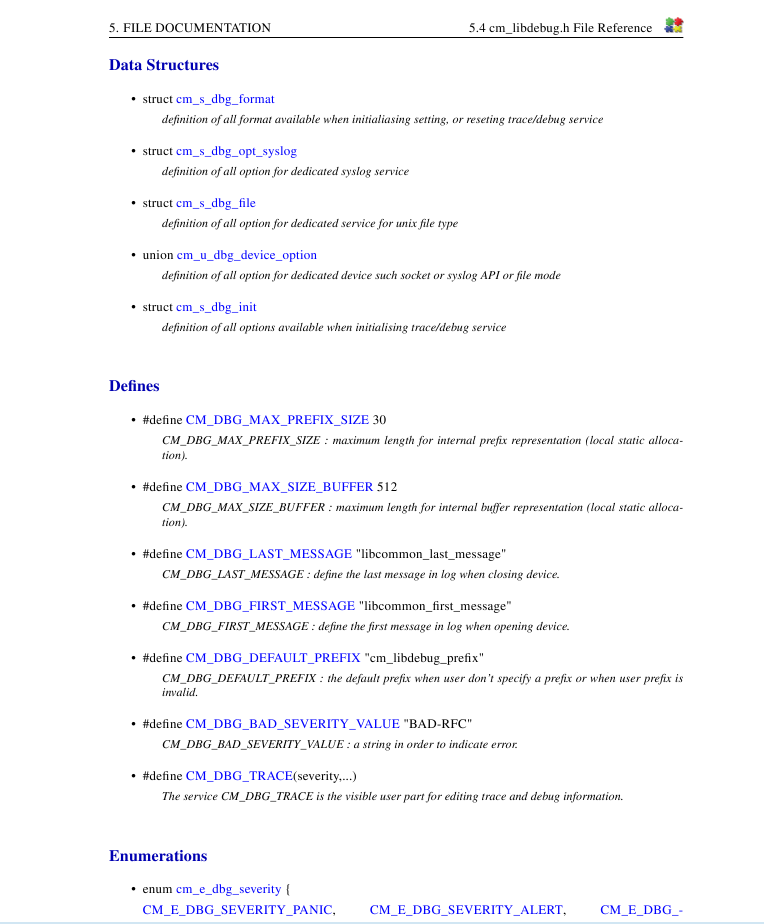
\includegraphics[width=12cm]{pictures/doxy_func}
\end{center}
\label{fig:doxy_output_1}
\caption{R�sultat du traitement des commentaires doxygen des fonctions et structures}
\end{figure}

\begin{figure}[ht]
\begin{center}
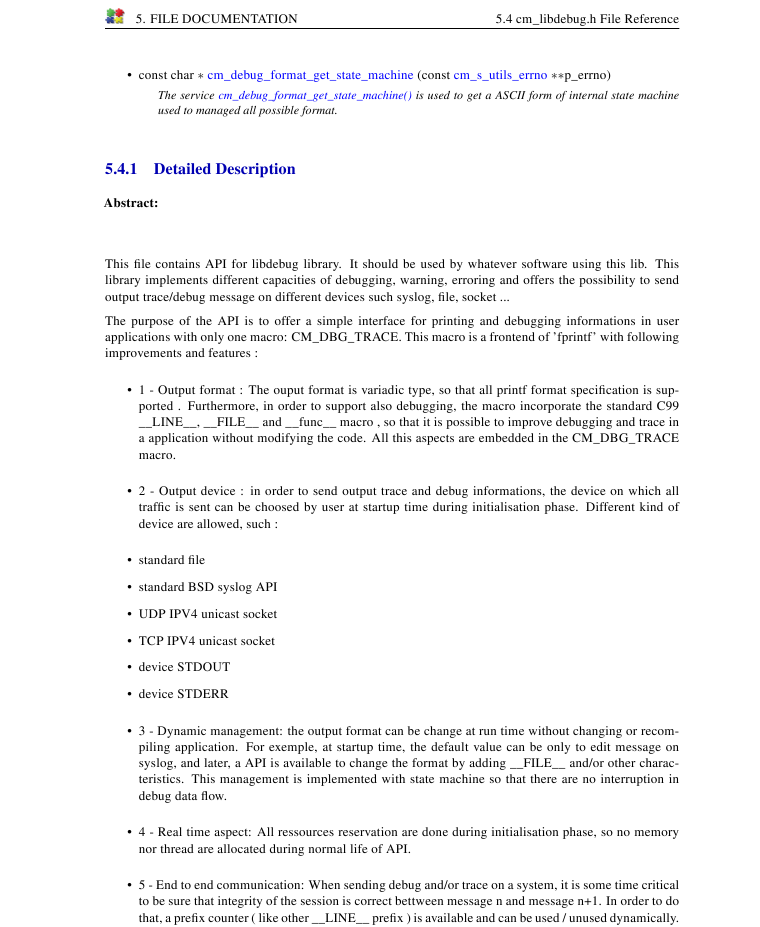
\includegraphics[width=12cm]{pictures/doxy_abstract}
\end{center}
\label{fig:doxy_output_2}
\caption{R�sultat du traitement de l'abstract du fichier srource}
\end{figure}


